%%%
%%% 	CHAPTER: INTRODUCTION 
%%%

% OUTLINE


	% OPENING
	
\section{Why study fluid mixing?}			
		
Fluid mixing happens in a gust of wind and in a cup of morning coffee with cream. This phenomena is commonplace and plays an important role in many natural and engineering systems that humanity depends on. Our current lack of fundamental understanding of mixing impedes our ability to understand natural systems such as atmospheric and oceanic processes that impact our global climate. Mixing also serves as a key industrial process crucial for production within the food, chemical, pharmaceutical, and petrochemical industries. Thoughtful design of industrial mixing is essential for maximizing product yield and product quality throughout these industries. In addition, poor mixing design can come at a cost. In 1989, the cost of poor mixing was estimated to be \$1 -- \$10 billion US dollars in the chemical industry alone \cite{paul2004handbook}. Nearly everyone depends on these industries for basic household products, health needs, travel, and food. And in most situations, the cost in production is inevitably paid by consumers --- that includes you and me. 


Although mixing is highly prevalent and often utilized, its fundamental principles are still not fully known especially concerning how the interplay of advection and diffusion processes affect mixing rates and achievable filamentation length scales. To make progress on understanding the systems that involve mixing, we must understand mixing itself. Thus, the approach taken here is to study a theoretical and mathematical framework of mixing that has been stripped down to its essential elements. The perspective taken in this work is that one must understand the idealized problems first before tackling problems with added complexity. An idealized Carnot engine provides efficiency expectations of real-world heat engines each unique with its own complexity. By analogy,  we hope the idealized mixer presented here will provide theoretical principles on mixing efficiency about real-world mixers as well.


\section{What does well-mixed mean?}

\begin{figure}
	\centering
	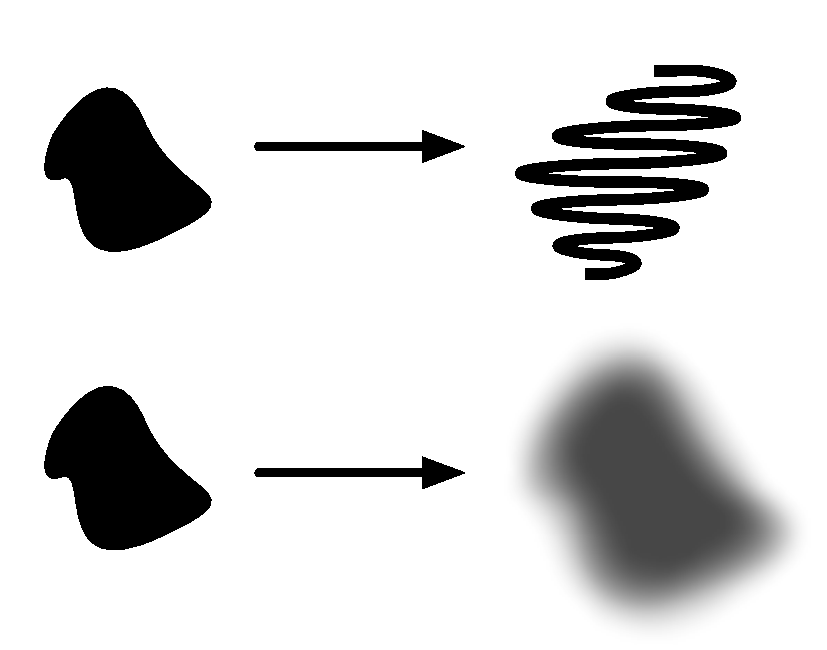
\includegraphics[width=0.7\textwidth]{ch-introduction/images/scale-and-intensity}
	\caption{Top transformation is a reduction in the scale of segregation. Bottom transformation is a reduction in the intensity of segregation}
	\label{fig:scale-and-intensity}
\end{figure}

In the pioneering work of P. V. Danckwerts (1952) \cite{Danckwerts1952}, the author identifies two indicators of mixed-ness: the scale of segregation and the intensity of segregation. The {\it scale of segregation } is the characteristic length scale present in the concentration. For instance, the process of thinning, elongating, and folding of a blob, as seen in the top graphic of figure \ref{fig:scale-and-intensity}, reduces the scale of segregation by creating a rich maze-like pattern with thin strands of dye.  The {\it intensity of segregation } refers to the variation of the concentration amplitude. This is naturally done by diffusion. The bottom graphic of figure \ref{fig:scale-and-intensity} shows a reduction in the overall variation and the concentration tends towards a state with a uniform concentration.





\section{Fluid mixing stages and mechanisms}

The seminal work of C. Eckart \cite{Eckart1948} describes the three stages of mixing:

\begin{enumerate}
\item {\it The initial stage}: The mixedness of the initial state will dictate the amount of `work' necessary to mix to a desired state. Typically, there will be large volumes of dye visible throughout the fluid.  Thus the preparation of the initial concentration is a stage in its own right before the fluid mechanisms are called into action.

\item {\it The intermediate stage}: {\it Advection}, or colloquially the act of stirring, will distort, stretch, and fold the volumes of dye to produce large gradients throughout the fluid and reduce the scale of segregation. 

\item {\it The final stage}: Lastly the gradients will disappear under the action of {\it diffusion}.  Diffusion refers to molecular diffusion throughout this work and not to be confused with its occasional usage of dispersal (to spread a dye thoughout space).  
\end{enumerate}
The intermediate and final stages are shown to happen sequentially in time. This is not completely accurate. These processes occur concurrently as we will investigate throughout this work.

In the stages above, we have introduced the two main mechanisms at play ---  advection and diffusion. Advection is a fluid mixing mechanism that when used appropriately can be an excellent way to reduce the scale of segregation. 

%Turbulent flows are commonly regarded as good mixers. In fact, its ability to mix may be considered a defining characteristic. To understand the impact of a turbulent flow on mixing, it is useful to examine the length scales present in the concentration field. This is commonly done through characterizing the scalar energy spectrum. The theory of Obukhoff (1949)\cite{Obukhov1949},  Corrsin (1951) \cite{Corrsin1951}, and Batchelor (1959)\cite{Batchelor1959a} captures the characteristics of the scalar energy cascades which have been verified numerically\cite{Eswaran1988,Holzer1994b,Shraiman2000a} and experimentally (CITATION). A key finding from their theory was the emergence of a length scale (now known as the Batchelor scale) where  advection and diffusion balance. The Batchelor scale is given by  $\ell_{b}= \sqrt{\kappa / \Gamma}$ where $\Gamma$ is the typical rate-of-strain of the fluid. For a turbulent flow to be sustained, there must be continual source of energy supplied to the fluid at the kinetic energy dissipation rate per unit mass $\epsilon$. This rate $\epsilon$ is related to the rate of strain $\Gamma = \langle |\nabla \mathbf{u}|^2 \rangle ^{1/2} $ by $\epsilon = \nu \Gamma^2$ where $\nu$ is the fluid viscosity \cite{Doering}. Using this relation, we find that the Batchelor scale is given by $\ell_{b}=\left(\frac{\kappa}{\nu}\right)^{1/2}\left(\nu^3/\epsilon\right)^{1/4}=S^{-\frac{1}{2}}\ell_{k}$ where $S=\frac{\nu}{\kappa}$ is the Schmidt number and  $\ell_{k}=\left(\nu^3/\epsilon\right)^{1/4}$ is the Kolmogorov length \cite{Dimotakis2005,Kolmogorov1941}.  The Batchelor scale defines the cutoff length in the scalar energy spectrum where there is rapid decay past this length according to the Obukhoff-Corrsin-Batchelor theory. Therefore, the presence of the Batchelor scale identifies a limit to the degree of mixing possible by a turbulent flow. 
	
\section{A mathematical framework for studying mixing}

The effect of advection and diffusion on the rate of fluid mixing depends on the particular mixing situation characterized by the unique fluid properties, specific mixing flow, and boundary geometry. In view of the vast complexity of the mixing situation, general principles of mixing underlying these various situations would be beneficial. In particular, it is valuable to determine how the mixing rate (typically the most optimal mixing rate) depends on aggregate flow intensity measures such as the stirring flows' energy and/or enstrophy. This is the objective of the research program encompassing many efforts \cite{CS2013,GI2014,JLT2012,JFM2011,  JLT2012, DF2014, GM2005,Yao2014a,JMP2012,Cortelezzi2008,Miles2018,Miles2017a} in last decade. 

With these goals in mind, a common approach taken throughout the literature is to consider the evolution of a tracer quantity $\theta$ advected by an incompressible ($\nabla \cdot\vec{u}=0$) flow $\vec{u}$ with mild physical constraints within a periodic box $D$ of side length $L$ in $d$ dimensions. All numerical simulations are done in 2 dimensions while analytical results are generally presented in arbitrary dimension. We will assume that $\theta$  has zero mean throughout this work. The tracer concentration field $\theta$ evolves according to the advection-diffusion equation,
\begin{equation}
	\label{eq:PDE_advection}
	\ppt{\theta}+\mathbf{u}\cdot \nabla \theta=\kappa \lap\theta,
\end{equation}
with initial data $\theta(\mathbf{x},0)=\theta_{0}(\mathbf{x})$, where $\kappa$ is the molecular diffusion coefficient and $\Delta = \nabla^2$ is the Laplacian operator. The flow intensity is constrained by enstrophy \begin{equation}
\ltwo{\nabla\u} = \sqrt{ \sint{|\nabla \mathbf{u}|^2} } =\Gamma L^{d/2}
\end{equation} or energy
\begin{equation} 
\ltwo{\u} = \sqrt{ \sint{| \mathbf{u}|^2} } = UL^{d/2}
\end{equation}
 where $\Gamma$ is the root mean square rate-of-strain and $U$ is the root mean square speed. We will also consider the time-average versions $\frac{1}{T}\int_0^T\ltwo{\nabla\u}^2 dt = \Gamma L^{d/2}$ or $\frac{1}{T}\int_0^T\ltwo{\u}^2 dt = U L^{d/2}$.


 The form above shows that the evolution of the tracer concentration $\theta$ is slaved to a given flow $\mathbf{u}$ which embodies, in many cases, most of the complexity of a particular mixing problem. The details of $\mathbf{u}$ alone can be complicated since in natural settings $\mathbf{u}$ is a solution of the Navier-Stokes equations. Although flow situations can be vastly different, they can still share commonalities such as incompressibility and similar amount of total energy or enstrophy. Note that enstrophy is proportional to the dissipation power for Newtonian fluids. We will only consider flows constrained by these properties for the purposes of simplicity and generality.


The negative Sobelov norms $H^{-n}$ \cite{GM2005, Mathew2007b,JLT2012, JFM2011} are measures of mixing used throughout the literature and the $H^{-1}$ norm (and sometimes referred to as the mix-norm) will be used here. The $H^{-n}$ norm for mean-zero scalar fields $\theta$ are given by  
%
\begin{equation}
\|\theta\|_{H^{-n}}=\ltwo{\nabla^{-n}\theta}=\sqrt{\sint{ |\nabla^{-n} \theta( \vec{x},t)|^2}}=\sqrt{ \sum_{\vec{k}\neq \vec{0}} L^d \frac{|\hat{\theta}_{\vec{k}}(t)|^{2}}{|\vec{k}|^{2n}}}
\end{equation}
%
where $\nabla^{-1}=\nabla \Delta^{-1}$, the operator $\Delta^{-1}$ acting on  a function $\rho$ returns the solution $\phi$ of the Poisson equation $ \Delta \phi = \rho $, and $\hat{\theta}_{\vec{k}}(t) =  \frac{1}{L^{d}}\sint{\theta(\vec{x},t)e^{-i\vec{k}\cdot\vec{x}}}$.  Lower values of the  $H^{-1}$ norm correspond to a more mixed state. Note that $H^{-1}$ norm can decrease in two ways. The first way is to decreasing the amplitudes of $|\hat{\theta}_{\vec{k}}|$ for $\vec{k}\neq 0$. This matches our first sense of mixing --- {\it homogenization}. The second way is by transferring spectral mass from the lower wave numbers to the higher wave numbers to take advantage of the $1/|\vec{k}|^2$ weighting of amplitudes at different length scales. This produces a scalar field with sharp gradients and small length scales which matches our second sense of mixing --- {\it filamentation}. Thus we can see that the $H^{-1}$ norm embodies both senses. 

The $L^{2}$ norm $\ltwo{\theta}$ defined by
%
\begin{equation}
\ltwo{\theta}=\sqrt{\sint{ | \theta( \vec{x},t)|^2}}=\sqrt{ \sum_{\vec{k}} L^d |\hat{\theta}_{\vec{k}}(t)|^{2}}
\end{equation}
%
and the $H^{1}$ norm $\hone{\theta}$ defined by 
%
\begin{equation}
\|\theta\|_{H^{1}} = \hone{\theta}=\sqrt{\sint{ |\nabla^{-1} \theta( \vec{x},t)|^2}}=\sqrt{ \sum_{\vec{k}} L^d |\vec{k}|^2|\hat{\theta}_{\vec{k}}(t)|^{2}}
\end{equation}
%
are also common measures of mixing and will be considered as well.  For those interested in other measures of mixing, see \cite{JLT2012}. 

			
\section{Pure diffusive mixing}
In the case without advection ($\vec{u}=\vec{0}$), equation \eqref{eq:PDE_advection} reduces to the classical heat equation \cite{Evans2010}. The Fourier modes evolve according to $\hat{\theta}_{\vec{k}}(t)=\hat{\theta}_{\vec{k}}(0)e^{-\kappa|\vec{k}|^2t}$. Thus we have explicit analytical results for the decay of the $H^{-1}$ norm by simply substituting this result. Note that $H^{-1}$ norm will surely decay monotonically since the amplitude of each mode does. Diffusion is unable to transfer spectral mass from the low wave number modes to the high wave number modes and thus is incapable of filamentation. Thus the pure diffusion case solely exploits homogenization. Also notice the unequal weighting attach to each mode. The Fourier modes with large wave number $|\vec{k}|$ decay at a much faster rate relative to the decay of those with small wave number.



\section{Pure advective mixing}
In the case without diffusion ($\kappa = 0$), pure advection of the flow is the only method of mixing, colloquially known as stirring. For a flow that is constrained by enstrophy, the mix-norm decays at most exponentially where the exponential rate is proportional to $\Gamma$ \cite{GI2014,CS2013}. This was mathematically proven by two separate approaches: G. Iyer {\it et. al.} \cite{GI2014} used regularization results of partial differential equations \cite{Crippa} while C. Seis \cite{CS2013} used methods from optimal transportation theory \cite{villani2003topics}. Furthermore, enstrophy-constrained flows that realize this exponential decay rate have been constructed analytically \cite{Alberti2014a}. On the other hand, energy-constrained flows can achieve even faster mixing rates. In fact they can achieve {\it perfect mixing in finite time} which means that the $H^{-1}$ norm reaches zero in finite time as opposed to approaching zero in infinite time as exhibited in the case for enstrophy-constrained mixing. This can be demonstrated by a `checkerboard' flow \cite{JMP2012} where the mix-norm achieves perfect mixing in finite time via linear decay.  For either flow intensity constraint, note that $H^{-1}$ norm decreases by exclusively exploiting filamentation without homogenization. This is exactly opposite to the purely diffusive case.

Many works \cite{DAlessandro1999a, Liu2006, Mathew2007b, Cortelezzi2008, DF2014, JFM2011, JMP2012, Farazmand, Balasuriya2005, Hobbs1998, Vikhansky2002} have framed mixing enhancement in terms of optimization and optimal control theory. Mathew {\it et al.} \cite{Mathew2007b} studied pure advection of a concentration field by a velocity field $\mathbf{u}=\sum_{i=1}^{N}\alpha_{i}\mathbf{u}_{i}$ where $\{\mathbf{u}_{i}\}$ is a finite set of divergence-free velocity fields and $\{\alpha_{i}\}$ is a set of time-dependent weights. The weights $\{\alpha_{i}\}$ were chosen to minimize the final-time $H^{-1/2}$ mix-norm subject to a fixed value of action or equivalently a fixed value of time-averaged energy. Necessary conditions for optimality were numerically solved by conjugate gradient. The authors considered two examples each using $\mathbf{u}_{1}$ and $\mathbf{u}_{2}$ as given cellular flow velocity fields. In both examples, they found that the $H^{-1/2}$ norm of the computed concentration field decayed at an exponential rate. Furthermore, the authors demonstrated that the kinetic energy must be conserved at all moments in time due to optimality conditions even though they only required that the {\it time-averaged} energy be fixed --- analogous results hold true in this work as well. For this particular choice of velocity fields, the enstrophy turns out to also be conserved. This is consistent with other theoretical and numerical works \cite{CS2013,GI2014,JFM2011,Alberti2014a} reporting exponential decay rates under fixed enstrophy.   

Cortelezzi {\it et al.} \cite{Cortelezzi2008} also considered controlling two given flows to enhance mixing. But rather than considering a superposition of two flows, the authors considered switching entirely between one flow and the other. In particular, the authors considered controls that picked one of two sine flows $\mathbf{u}_{1}=\sin(2\pi y)\hat{x}$ and $\mathbf{u}_{2}=\sin(2\pi x)\hat{y}$ at uniformly spaced switching times. The authors divided the optimization task into multiple optimization sub-problems performed over short time horizons covering the entire time interval. They found, in the presence and absence of diffusion, that the mixing efficiency, as measured by the $H^{-1/2}$ mix-norm, of the short-horizon optimization schemes was substantially better than the periodic control that alternates between the two flows at each switching time. They also concluded that mixing can be greatly enhanced when optimizing over very short time horizons.
 
 Lin {\it et al.} \cite{JFM2011} explored short-time considerations even further. They found an analytic expression for the instantaneous optimal choice of velocity field given the current concentration field under fixed energy and enstrophy constraints. This was done by minimizing the time derivative of the $H^{-1}$ norm at each instant. Using the resulting expression, they numerically integrated the advection equation forward in time while determining the optimal velocity field at each time step. For an enstrophy-constrained flow, they numerically demonstrated exponential decay of the $H^{-1/2}$ and $H^{-1}$ norms consistent with \cite{CS2013,GI2014,Alberti2014a,Mathew2007b}. Lunasin {\it et al.} \cite{JMP2012} also performed a similar analysis as Lin {\it et al.} for flows with fixed palenstrophy ($\|\Delta\mathbf{u}\|_{L^{2}}$). This form of optimization is referred to as local-in-time optimization and will be discussed further shortly.


\section{The interplay of advection and diffusion}

Finally, the case with diffusion and advection is the least explored in this framework and the focus of this thesis. It is known that the evolution of the $H^{-1}$ and $L^2$ norms decrease monotonically under the checkerboard flow introduced by \cite{JMP2012}
 while the $H^{1}$ increases until it reaches a peak and then decreases \cite{DF2014}. This peak corresponds to a  time when the length scales developed are small enough for diffusion to effectively act on steep gradients. In contrast to the `pure' cases mentioned earlier, it is important to note that the $H^{-1}$ can now decrease by the two avenues of homogenization and filamentation simultaneously. 

At this point, we can already see a glimpse of a conflict between diffusion and advection for the ultimate goal of optimal mixing. Pure advection succeeds at filamentation by transferring spectral mass from the low wave number modes to the high wave number modes in a continuous fashion. However in the presence of diffusion, a once optimal pure advection flow exceptional at filamentation will be met with potential conflict since homogenization by diffusion can stifle its progress in transferring spectral mass to high wave number modes. Given that diffusion is ubiquitous, we must come to terms with this conflict to produce efficient mixing.


		
\section{The question and goals}

In this work, the interplay of advection and diffusion is explored to determine its impact on the rate of mixing. As we have mentioned in the last section, there appears to be a conflict between advection and diffusion that arises when both are acting to reduce homogenization through reduction in scale and intensity of segregation simultaneously.  The main question underlying this entire thesis work is:

\begin{quote}
{\it What is the optimal mixing rate achievable under the enstrophy and energy constrained flows when both advection and diffusion are active? }
\end{quote}

We hope to make progress in answering this by posing the question as an optimization problem. We will consider the {\it local-in-time optimization} problem:

\begin{equation} 
\min_{\vec{u}} \ddt{}\hmone{\theta(\cdot, t) }^2
\end{equation}
where the flow intensity is constrained by enstrophy \begin{equation}
\ltwo{\nabla\u}^2 =\Gamma^2 L^{d}
\end{equation} or energy
\begin{equation} 
\ltwo{\u}^2 = U^2L^{d}.
\end{equation}
%
We also consider the {\it global-in-time optimization } problem:
%
\begin{equation} 
\min_{\vec{u}} \hmone{\theta (\cdot, T) }^2
\end{equation}
%
where the flow intensity is constrained by {\it time-averaged} enstrophy \begin{equation}
\frac{1}{T}\int_0^T\ltwo{\nabla\u}^2 = \Gamma^2 L^{d}
\end{equation} or time-averaged energy
\begin{equation} 
\frac{1}{T}\int_0^T \ltwo{\u}^2 = U^2L^{d}.
\end{equation}

For all formulations, the flow is always required to be divergence-free ($\nabla \cdot \mathbf{u} = 0$) and $\theta$ solves the advection-diffusion equation with initial data $\theta(\mathbf{x},0)=\theta_0(\mathbf{x})$.

%
%\section{Feasibility of optimal flows}
%
%It is natural to ask ``Are optimal flows as defined feasible?" and ``How would one generate such flows in reality?" The purpose of this study is not to tackle these questions directly since our formulation is not entirely suitable for these questions. The purpose of this study is to consider idealized mixing to provide expectations in the best-case scenario with absolute control over the velocity field under the assigned constraints. In reality absolute control is generally not obtainable. As mentioned in the Carnot engine analogy discussed earlier in this chapter, the Carnot engine is an idealized engine with efficiency expectations in the best-case scenario which bound realizable engines, the approach taken here is similar. We hope to construct idealized mixers with mixing efficiency exceptions that bound realizable flows with known flow intensities quantified by energy and enstrophy.
%
%Although we do not fully address feasibility in the series of studies presented here, we acknowledge that feasibility is an important issue and encourage research in this direction. We will however say as much as we can in this section on the topic of feasibility to promote investigation. 
%
%With the goal of feasibility in mind, we can work backwards from a desired flow $\mathbf{u}$ to obtain the required forcing $\mathbf{f}$ on a fluid. This  can be found by simply substituting a discovered (local- or global-in-time) optimal velocity field $\mathbf{u}$ into the Navier-Stokes equation:
%\begin{equation}
%\label{eq:ns}
%\mathbf{f} = \rho\partial_{t} \mathbf{u}  + \rho\mathbf{u}\cdot \nabla \mathbf{u} + \nabla p - \nu \Delta \mathbf{u} 
%\end{equation}
%where $\rho$ is the fluid density, $\nu$ is the viscosity, $p$ is the fluid pressure, and $\mathbf{f}$ is the required forcing. Thus, we have obtained the necessary forcing to generate the desired flow $\mathbf{u}$. The next natural question is ``How could you construct a mixing device to create the forcing $\mathbf{f}$?'' Although we do not provide an answer, the derived forcing $\mathbf{f}$ at least gives us a target to aim for when tasked with the engineering problem of designing a mechanical mixer that realizes the flow $\mathbf{u}$. 
%
%%Note that the power injected by external forcing on fluid is eventually exhausted by viscous dissipation in the fluid. The viscous power dissipation rate is $\nu\int_{D}|\nabla \mathbf{u}|^2 \, d\mathbf{x}$
%
%The required mechanical power and energy to operate a mixing device are also useful measures for evaluating feasibility. For instance if the mechanical power or energy blows up in finite time, this would rule out it feasibility. The mechanical power $P$ can be found by multiplying \eqref{eq:ns} by $\mathbf{u}$ and integrating over the domain $D$ to arrive at
% \begin{equation}
%(P \equiv ) \sint{\mathbf{f}\cdot\mathbf{u}} = \ddt{}\left( \frac{\rho}{2}\sint{|\mathbf{u}|^2}\right) + \nu\sint{|\nabla\mathbf{u}|^2}
%\end{equation}
%where the left-hand side is identified as the mechanical power $P$ injected into the fluid by the external forcing $\mathbf{f}$, $ \frac{\rho}{2}\sint{|\mathbf{u}|^2}$ is the total kinetic energy, and $\sint{|\nabla\mathbf{u}|^2}$ is the enstrophy. 
%
%
%Under the enstrophy-constrained case, we have
%\begin{equation}
%P = \ddt{}\left( \frac{\rho}{2}\sint{|\mathbf{u}|^2}\right) + \nu\Gamma^2 L^d.
%\end{equation}
%The associated mechanical energy $E = \int_0^{T} P(t) dt$ is 
%\begin{equation}
%E = \left( \frac{\rho}{2}\sint{|\mathbf{u}(\mathbf{x},T)|^2} - \frac{\rho}{2}\sint{|\mathbf{u}(\mathbf{x},0)|^2}\right) + \nu\Gamma^2 L^d T.
%\end{equation}
%By Poincare's inequality we find that 
%\[
%E \leq \frac{\rho}{4\pi}\Gamma^2L^{d+2}  + \nu \Gamma^2L^dT.
%\]
%Thus, we see that the mechanical power $P$ required over time depends on the rate of total kinetic energy associated with the flow $\mathbf{u}$. However, the total mechanical energy $E$ is guaranteed to stay bounded from above by a quantity linearly proportional to enstrophy quantified by $\Gamma^2 L^d$.  Although the construction of a mechanical mixer enforcing $\mathbf{f}$ remains a challenge, the amount of mechanical energy required to enforce the enstrophy constraint is sensible --- in the sense that the above energetic analysis does not rule out its physical feasibility (the mechanical energy $E$ does not diverge in time for instance). 
%
%
% Under the energy-constrained case, the mechanical power is
%\begin{equation}
%\label{eq:energy-power}
%P = \nu\sint{|\nabla\mathbf{u}|^2}
%\end{equation} 
%and the mechanical energy is
%\begin{equation}
%\label{eq:energy-energy}
%E = \nu\int_0^{T}\sint{|\nabla\mathbf{u}|^2}dt
%\end{equation} 
%Thus, the amount of mechanical power is proportional to the amount of enstrophy or viscous energy dissipation rate. The development of small length scales is not penalized under energy-constrained flows thus this could result in \eqref{eq:energy-power} growing over time. This will certainly be the case under the checkerboard flow without diffusion. In the case with diffusion, we will demonstrate in later chapters the presence of a limiting length scale in the concentration field $\theta$ proportional to a generalized Batchelor scale $\lambda_{U} = \frac{\kappa}{U}$. For the present analysis, note that it does not seem beneficial for mixing to generate length scales in the velocity field significantly smaller than those present in the concentration field.  If we assume that the Fourier spectrum is peaked around the wavenumber $\frac{2\pi}{\lambda_{U}}$ at later times after the developing the smallest length scale $\lambda_U$. Then, we hypothesize that, during this later stage, the mechanical power scales according to 
%\begin{equation}
%\label{eq:power-expectation}
%P \sim \nu \frac{(2\pi)^2}{\lambda_{B}^2}U^2 L^d  = \nu \frac{(2\pi)^2}{\kappa^2}U^4 L^d.
%\end{equation}
%Note the scaling with $\nu$, $\kappa$, and $U$. As $\kappa$ decreases, this increases the mechanical power. We will see in later chapters that a decrease in $\kappa$ is also accompanied by a beneficial {\it increase} in the mixing rate. Thus, this presents a trade off between these potential objectives: mixing efficiency and mechanical power. 
%
%In both enstrophy- and energy- constrained cases, it is beneficial to have a lower viscosity $\nu$. This is especially important for the energy-constrained case where the mechanical power is proportional to $\nu$.

\section{Organization of dissertation}
The rest of this dissertation is organized as follows:  Chapter \ref{chap:shellmodel} describes the local- and global-in-time optimization within the context of a shell model, a model representing the spectral dynamics of the advection-diffusion equation. Here we find the first indication that diffusion in some cases can penalize mixing performance. This work was published in the Journal of Nonlinear Science in 2017 \cite{Miles2017a}. Chapter \ref{chap:lit} studies local-in-time optimization in the context of the advection-diffusion partial differential equation. Here we investigate further the impact of diffusion. We find that diffusion can in some cases negatively impact the long-term mixing rate for local-in-time optimal flows. This work has been accepted for publication in Nonlinearity \cite{Miles2018}. Chapter \ref{chap:git} presents on-going work on global-in-time optimization of the advection-diffusion equation. An analytical result is presented showing that it is optimal to expend the stirring budget uniformly in time for the pure advection case. This result appears in an Appendix section of the 2017 Journal of Nonlinear Science article \cite{Miles2017a}.

%	
%	These problems are explored in the context of the shell model in chapter \ref{chap:shellmodel}. They are explored further in the context of the advection-diffusion equation in chapters \ref{chap:lit} and \ref{chap:git}.




% SCRATCHWORK BELOW

%Many have explored the idea of enhancing mixing by stirring.  Eckart (1948) is one of the earliest to explore this topic. He argued that there are three mixing stages: initial stage (persistance of large scales in initial concentration), intermediate stage (the creation of gradients induced by advection), and final stage (the disappearance of gradients by diffusion). He explored these phases in the simplified setting of a planar shear flow and concluded that the mixing times occurred on the order of $t=\ell^{2}/\kappa$ where $\ell$ is the length scale of the velocity field. Thus, Eckart was one of the first to quantify the impact of the velocity length scale on the concentration mixing rate.
%
%\section{turbulence}
%

%
%
%Mixing enhancement through optimization and optimal control techinques have been explored\cite{Mathew2007b,Cortelezzi2008,Liu2006, JFM2011}.
